\documentclass{article}
\usepackage{graphicx}

\begin{document}
\graphicspath{ {./images/} }

\title{This is documentation for present my website project} 
\author{Mohammad Abdallh}
\maketitle

\begin{abstract}
 This website is divided into a group of sections to help you reach whatever your goal is and help you to start developing once you choose your own path it will lead you to start your own buisnes for being more creative and able you to be updated with the outer world
\end{abstract}

\section{Introduction}
If you want to become one of the most important programmers right now, and have your own successful buisness this site is the best for you this is the website for group of courses such as cyber security , web design ,It,data analysis and app development.we divided our website into group of sections with html , css , javascript languages and in this introduction we will discuss fluently every page If you want to become one of the most important programmers right now, and have your own successful buisness this site is the best for you this is the website for group of courses such as cyber security , web design ,It,data analysis and app development.we divided our website into group of sections with html , css , javascript languages and in this introduction we will discuss fluently every page:

\begin{itemize}
\item Home page 
\item About page 
\item Blog page
\item Service page
\end{itemize}


\section{Home Page}
the home page contains details about our website such as the clients that joined us , the number of projects done by our previous clients , group of articles of each path as a little intro for it fegure (\ref{fig:home})

\begin{figure}
\centering

\includegraphics[scale=.2]{images/home.png}
\label{fig:home}
\caption{This photo describe home page}
\end{figure}

\section{service page}

the service page contains our courses that will help you find your path and reviewes from our previous clients figure (\ref{fig:service})

\begin{figure}
\centering
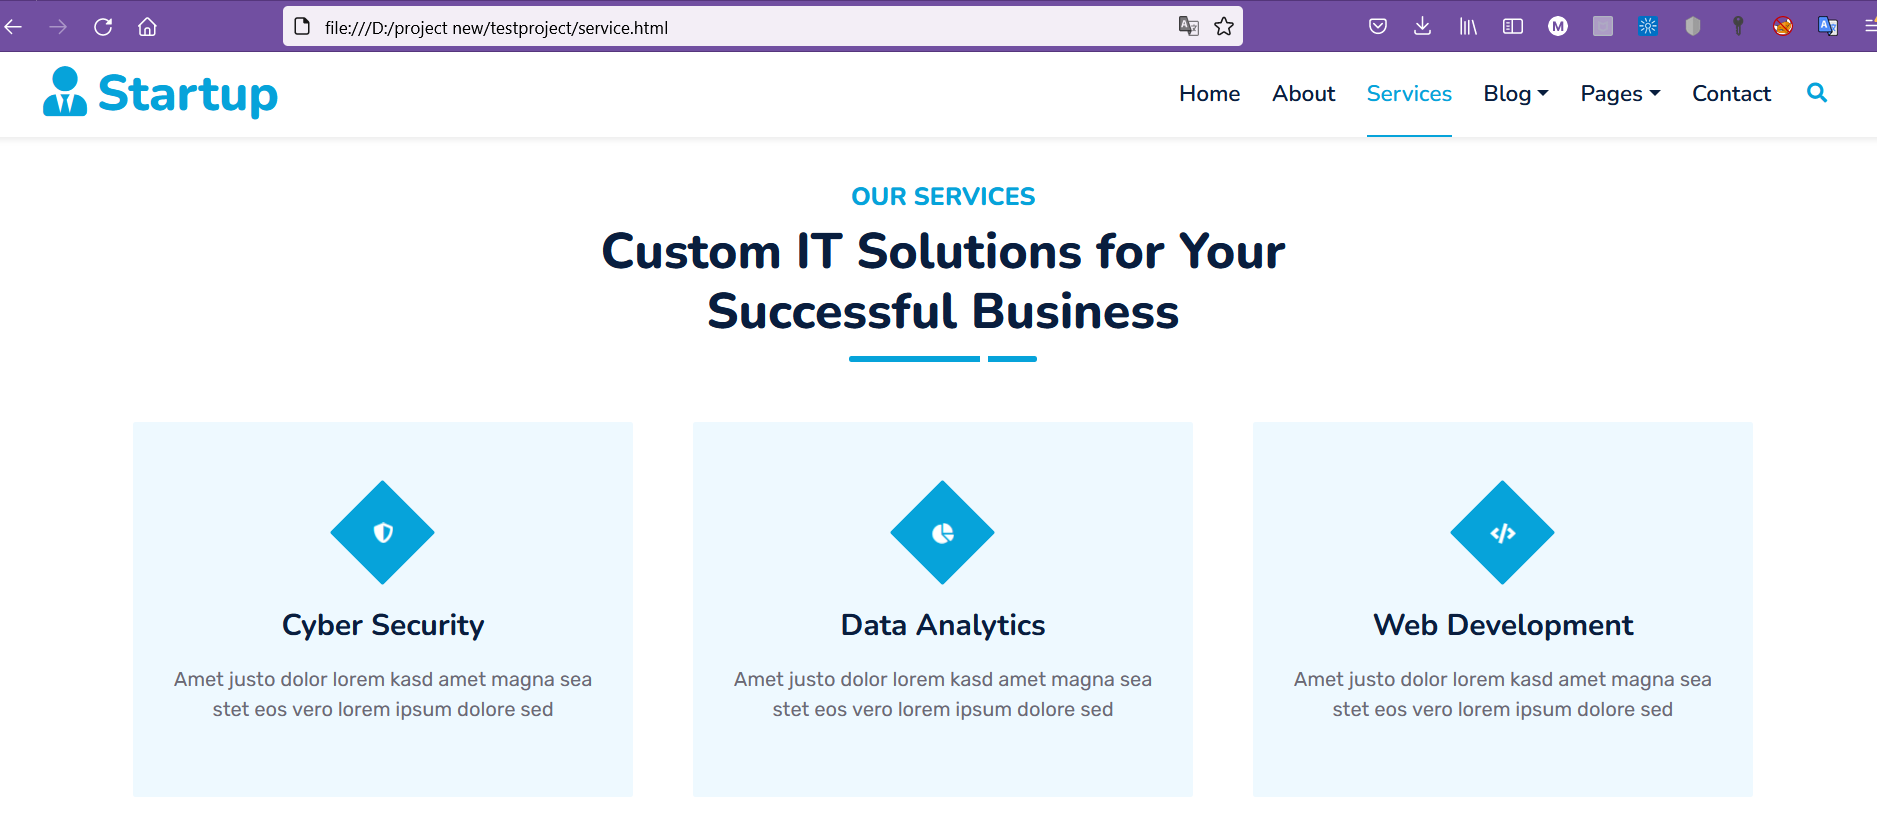
\includegraphics[scale=.2]{images/service.png}
\label{fig:service}
\caption{This photo describe service page}
\end{figure}

\section{Blog page}
\subsection{blog gride}
This page helps to choose which plans we can follow to achieve the best result figrue (\ref{fig:blog} ).
\subsection{blog detail}
this section you choose your path and you log in and leave your own comment or review for the projects figure (\ref{fig:bloggrid} ).

\begin{figure}
\centering
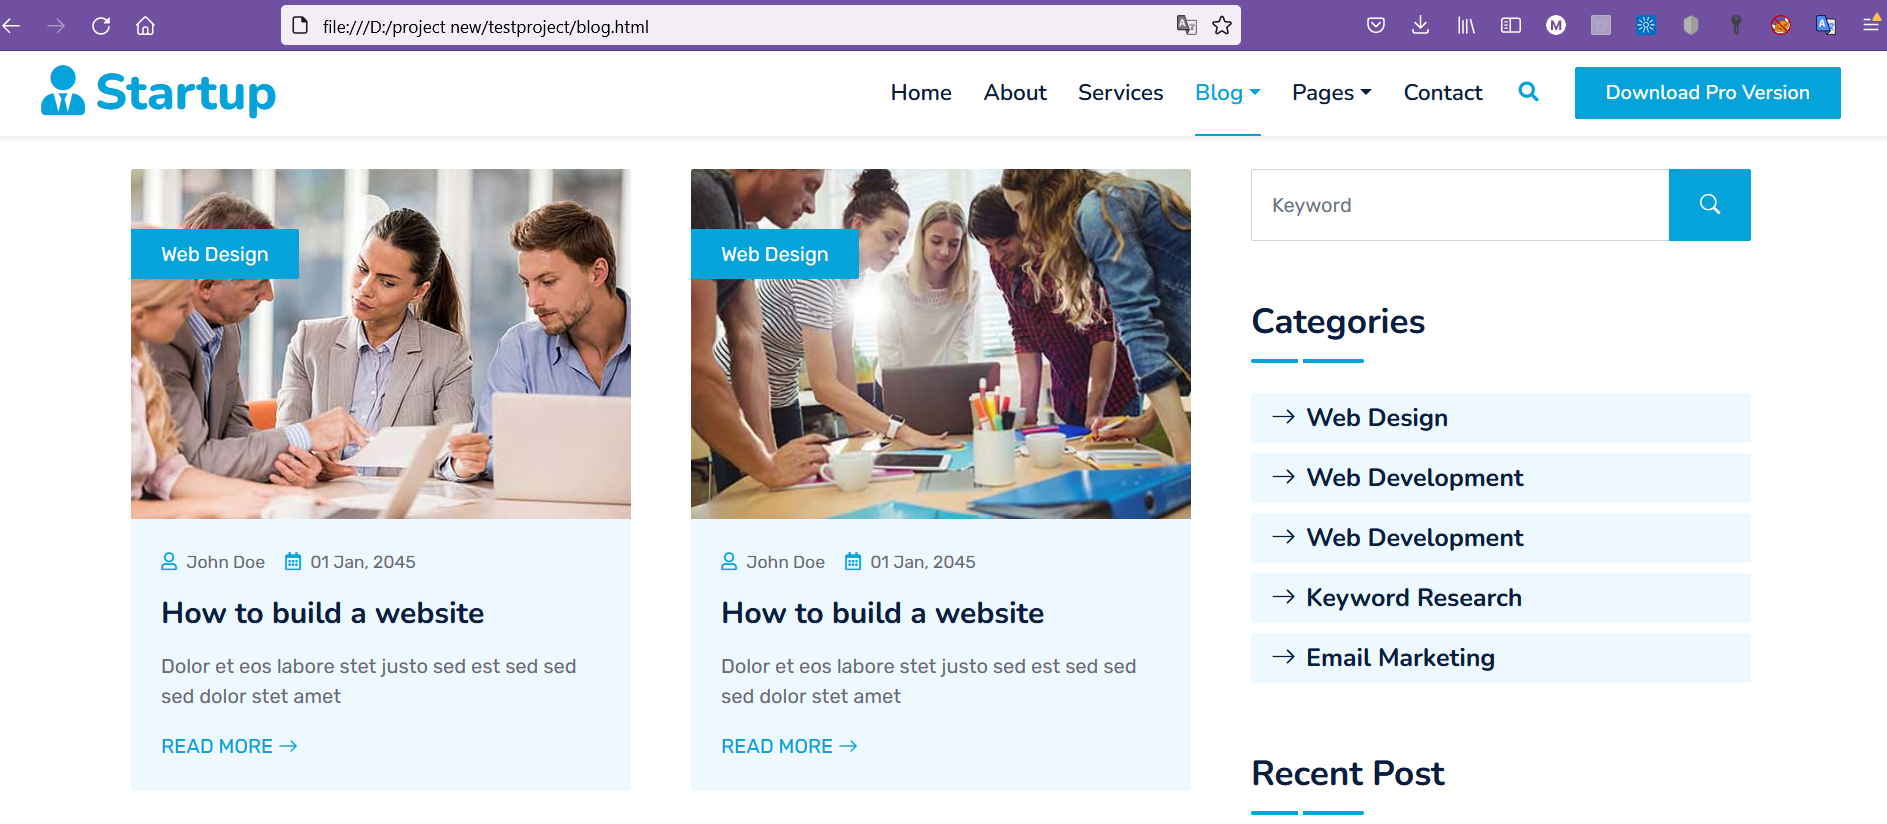
\includegraphics[scale=.2]{images/blog.png}
\label{fig:blog}
\caption{This photo describe blog page }
\end{figure}

\begin{figure}
\centering
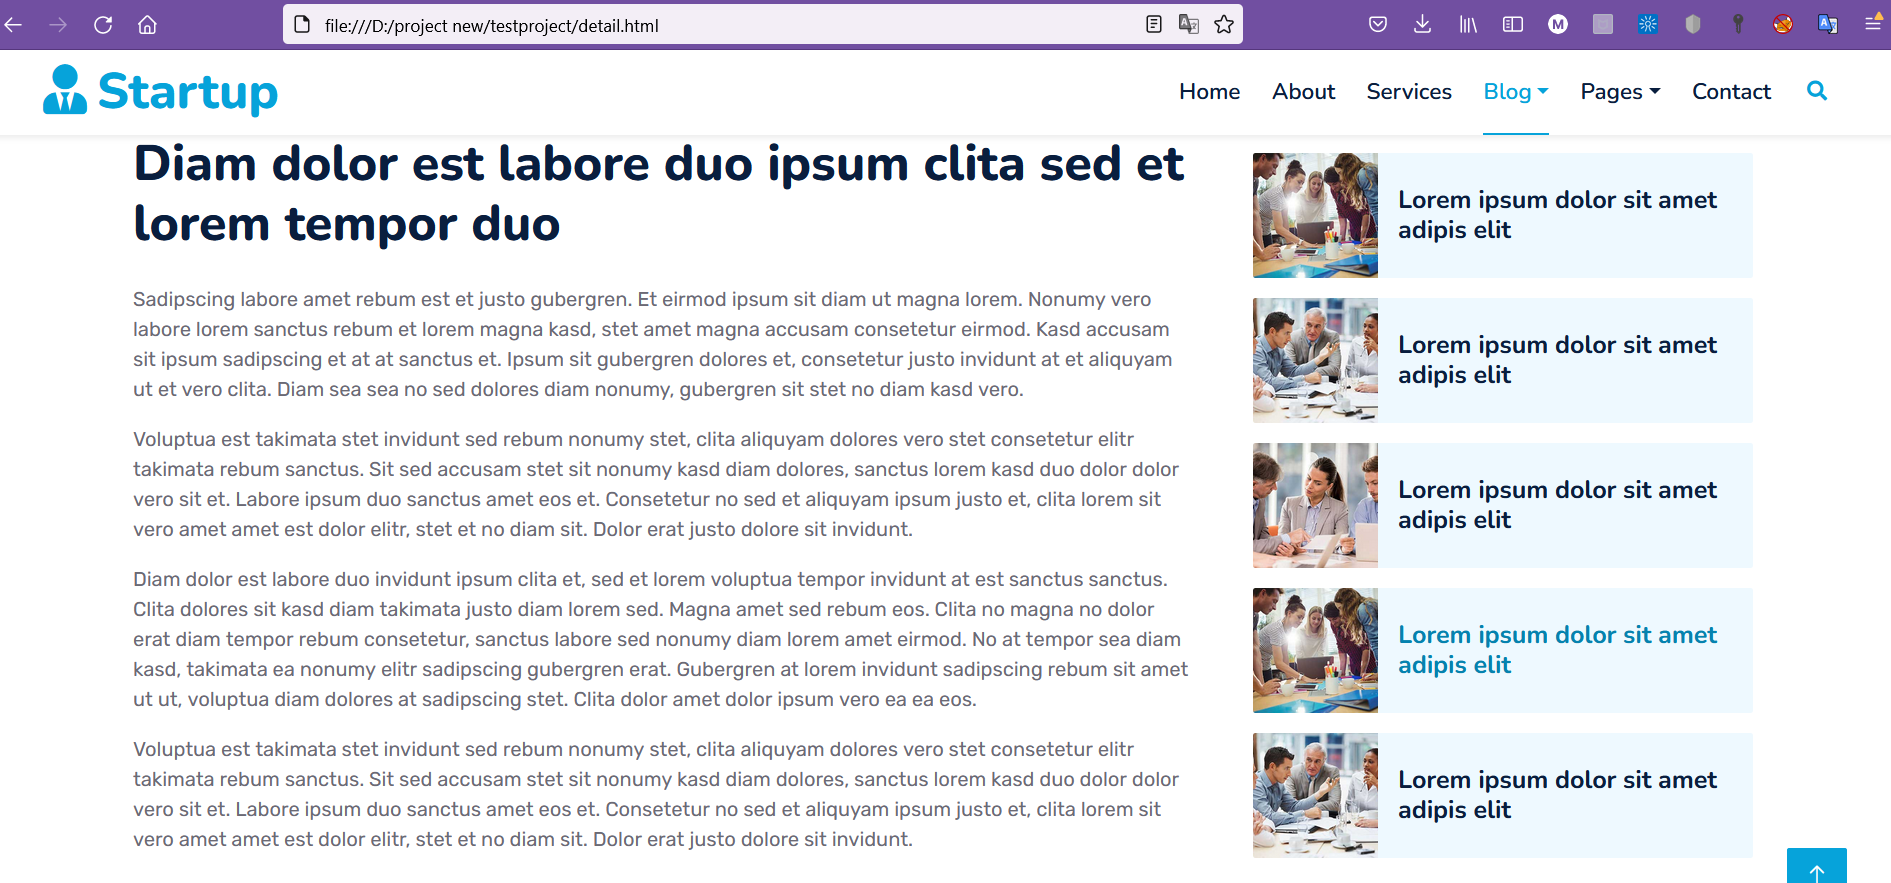
\includegraphics[scale=.2]{images/bloggrid.png}
\label{fig:bloggrid}
\caption{This photo describe blog grid page }
\end{figure}


\section{about page}
the about page helps you to know who we are, what experiences we have , the offers we have for you to be with us , our number and our creative team members that will help you start your own buisness figure( \ref{fig:about} ).

\begin{figure}
\centering
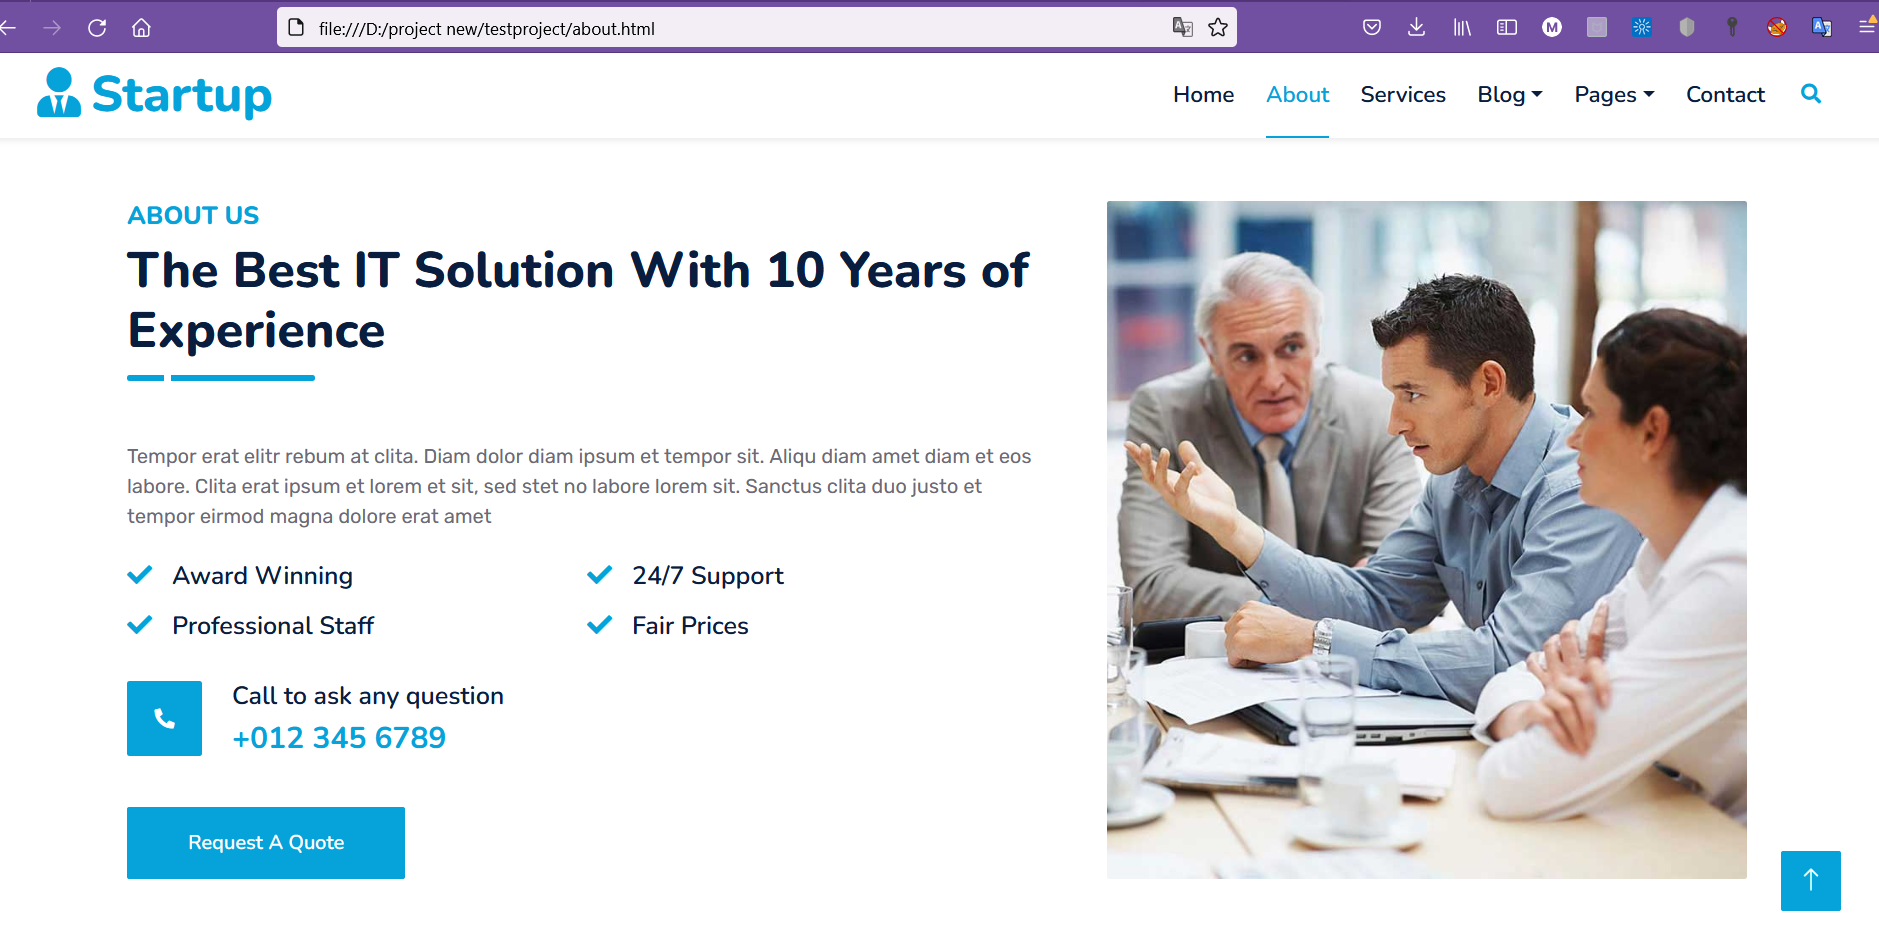
\includegraphics[scale=.2]{images/about.png}
\label{fig:about}
\caption{This photo describe about page}
\end{figure}

\section{contact}
In this page we leave you with ways of how to contact us by using our phone number and if you want leave us a message you can use our email or you can visit our branch figure( \ref{fig:contact} ).

\begin{figure}
\centering
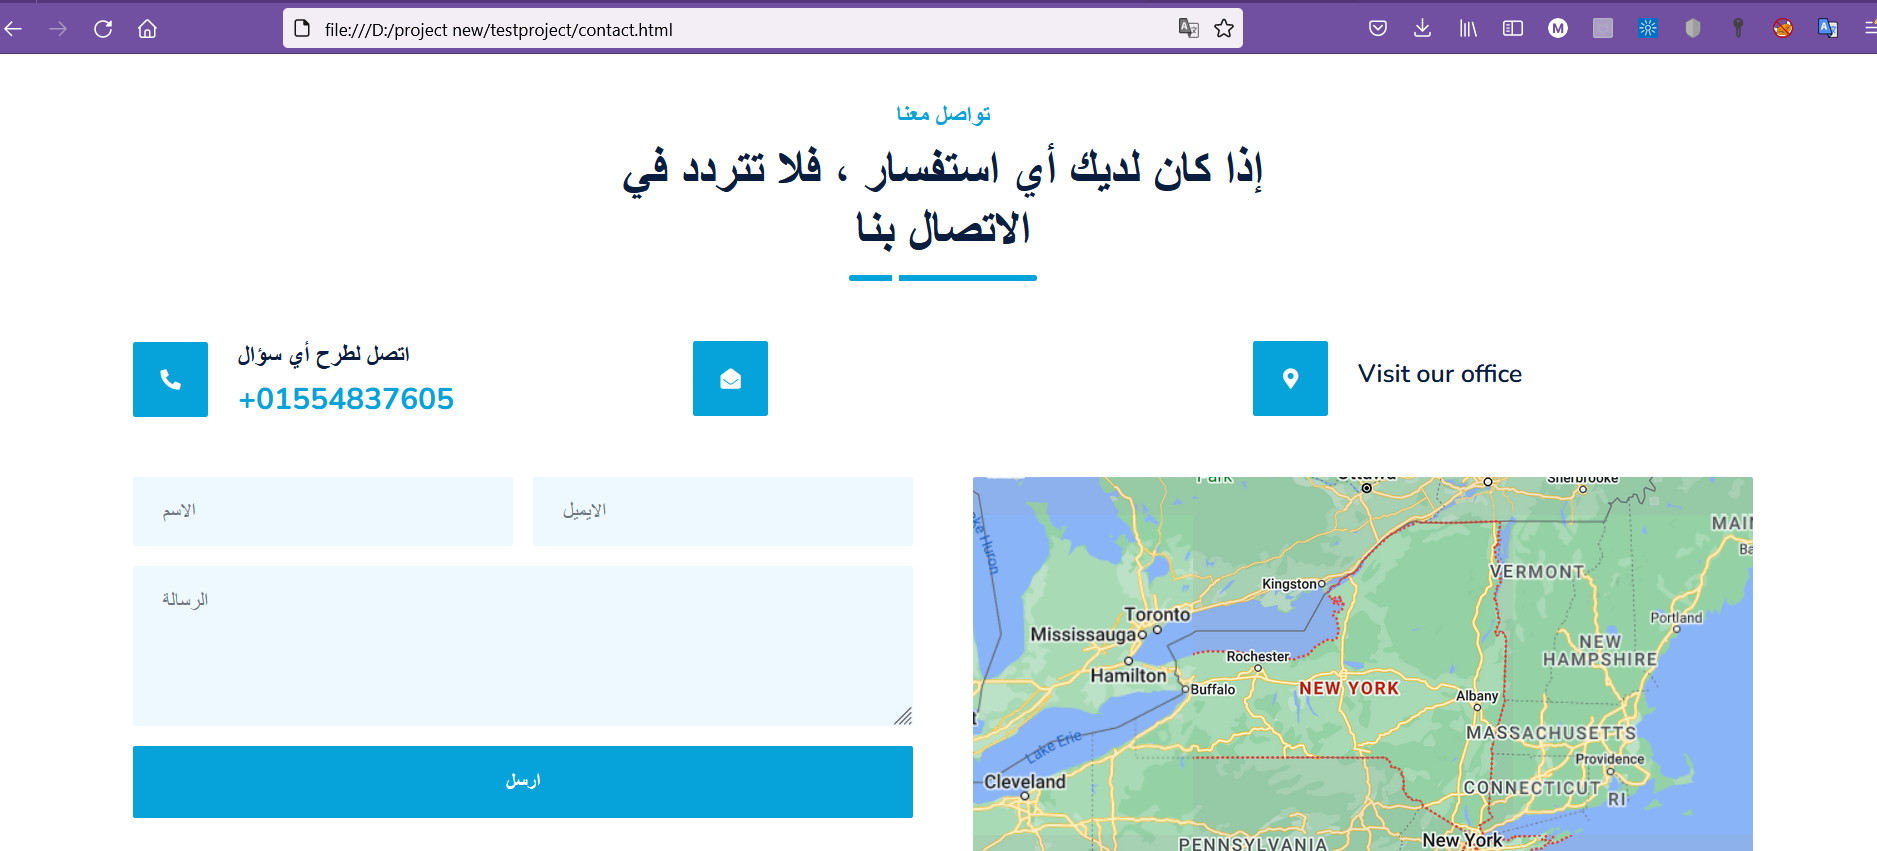
\includegraphics[scale=.2]{images/contact.png}
\label{fig:contact}
\caption{This photo describe contact }
\end{figure}

\section{conclusion}
If you want to become one of the most important programmers right now, and have your own successful buisness this site is the best for you this is the website for group of courses such as cyber security , web design ,It,data analysis and app development.we divided our website into group of sections with html , css , javascript languages and in this introduction we will discuss fluently every page If you want to become one of the most important programmers right now, and have your own successful buisness this site is the best for you this is the website for group of courses such as cyber security , web design ,It,data analysis and app development.we divided our website into group of sections with html , css , javascript languages and in this introduction we will discuss fluently every page
\begin{table}
\centering
\caption{this is table show each one what do in project}
\label{table:myteam}
\begin{tabular}{r | c r}
	\hline
	No. & Name & page \\
	\hline
	1 & \textbf{Mohammed Abdallh} & service \\
	2 & Mohammed Mossad  & price \\
	3 & Mohammed Ayman & home \\
	4 & Rahma Hussein  & javaScript \\
    5 & Omnya Ahmed & blog \\
	6 & Sara Atef  & about \\
	\hline
\end{tabular}
\end{table}

\section{My team}
\begin{enumerate}
\item Mohammed abdallh 
\item omnya Ahmed 
\item Sara atef 
\item Rahma Hussien 
\item Mohammed Mossad 
\item Mohammed Ayman
\end{enumerate}

\end{document}